%% PNAStwoS.tex 
%% Sample file to use for PNAS articles prepared in LaTeX 
%% For two column PNAS articles %% Version: Apr 15, 2008
 
%% BASIC CLASS FILE 
\documentclass{pnastwo}
%% ADDITIONAL OPTIONAL STYLE FILES 
\usepackage[dvips]{graphicx}
\usepackage{pnastwoF} 
\usepackage{amssymb,amsfonts,amsmath} 
\usepackage{url}
%\bibliographystyle{pnas2009}

%% OPTIONAL MACRO DEFINITIONS 
\def\s{\sigma} 
\usepackage{url}
\begin{document}

\title{Tackling soil diversity with the assembly of large, complex metagenomes}

\author{Adina Chuang Howe\affil{1}{Microbiology and Molecular Genetics, Michigan
State University, East Lansing, MI, USA}\affil{2}{Plant, Soil, and Microbial
Sciences,Michigan State University, East Lansing, MI, USA}, Janet
Jansson\affil{3}{Department of Energy (DOE) Joint Genome Institute, Walnut
Creek, CA, USA}\affil{4}{Lawrence Berkeley National Laboratory, Earth Sciences
Division, Berkeley, CA, USA}, Stephanie A. Malfatti\affil{3}{}, Susannah G.
Tringe\affil{3}{}, James M. Tiedje\affil{1}{}\affil{2}{}, and C. Titus
Brown\affil{1}{}\affil{5}{Computer Science and Engineering, Michigan State
University}}

\contributor{Submitted to Proceedings of the National Academy of Sciences of the
United States of America} \maketitle

\begin{article} \begin{abstract} The large volumes of sequencing data required
to sample complex environments deeply pose new challenges to sequence analysis
approaches. De novo metagenomic assembly effectively reduces the total amount of
data to be analyzed but requires significant computational resources. We apply
two pre-assembly filtering approaches, digital normalization and partitioning,
to make large metagenome assemblies more computationally tractable. Using a
human gut mock community dataset, we demonstrate that these methods result in
assemblies nearly identical to assemblies from unprocessed data. We then
assemble two large soil metagenomes from matched Iowa corn and native prairie
soils and investigate the functional potential of these soils.  The
assembly strategies presented are generic and can be extended to any metagenome
and any assembler; full source code is freely available under a BSD license.
\end{abstract}

\keywords{assembly | soil | metagenomics}

\dropcap{C}omplex microbial communities operate at the heart of many crucial
terrestrial, aquatic,and host-associated processes, providing critical ecosystem
functionality that underpins much of biology
\cite{Arumugam:2011p735,Hess:2011p686,Iverson:2012p1281,
Mackelprang:2011p1087,Qin:2010p189,Tringe:2005p174,Venter:2004p170}. DNA
sequencing has begun to reveal the enormous diversity and heterogeneity
associated within these systems, making them difficult to study {\em in situ}
\cite{Hess:2011p686,Mackelprang:2011p1087,Qin:2010p189}. With ultradeep
sequencing, we now have unprecedented access to even the rare species in these
environments though with large volumes of sequencing (i.e., ~50 Tbp required to adequately sample a gram of soil
\cite{Gans:2005p1365}).

Alongside sequencing breakthroughs, new challenges to sequence analysis
approaches have emerged. Sequencing dataset sizes are growing at an exponential
rate, requiring significant computational resources for data storage and
analysis. A single metagenomic project can readily generate as much or more data
than is in global reference databases; for example, a human-gut metagenome sample
containing 578 Gbp \cite{Qin:2010p189} produced more than double the data in NCBI
RefSeq (Release 56). Moreover, short reads contain only minimal signal for
homology searches and are error-prone, limiting direct annotation approaches
against reference databases. And finally, the majority of genes sequenced from
complex metagenomes typically contain little or no similarity to experimentally
studied genes, further complicating homology analysis
\cite{Arumugam:2011p735,Qin:2010p189}.

Consequently, investigators of metagenomic datasets are confounded by
overwhelming volumes of data for which they do not have the computational resources
to efficiently analyze or which are unsuitable for the current suite of
bioinformatic tools (because of short read lengths or a lack of reference
genomes). \emph{De novo} assembly of sequence data offers several advantages for
analyzing metagenomic datasets. It provides improved accuracy of sequences by
removing most random sequencing errors and results in contigs longer and more
specific than unassembled sequencing reads. Further, assembly significantly
reduces the total volume of data required for downstream analysis (e.g., gene
annotation). Importantly, \emph{de novo} assembly also does not rely on the
existence of reference genomes, thus allowing for the discovery of novel genomic
elements. The main challenge for metagenomic applications of \emph{de novo}
assembly is that current assembly tools do not scale to the high diversity and
large volume of metagenomic data: metagenomes from rumen, human gut, and
permafrost soil sequencing could only be assembled by discarding low abundance
sequences prior to assembly
\cite{Hess:2011p686,Mackelprang:2011p1087,Qin:2010p189}. Although many
metagenome-specific assemblers have recently been developed for community
assembly, they cannot work with the volume of reads necessary to achieve high
coverage for extremely diverse environmental metagenomes
\cite{metaray, Scholz:2012p1372}.

Here, we present two pre-assembly read filtering strategies, digital
normalization and partitioning, that provide a general strategy for scaling and
improving metagenome assembly. Digital normalization normalizes sequence
coverage and reduces the dataset size by setting aside reads from high-coverage
regions. Subsequently, partitioning separates reads based
on transitive connectivity, resulting in easily assembled subsets of reads. 
We evaluate these approaches by applying them
to a human gut mock community (HGMC) dataset and find that these filtering
methods result in assemblies nearly identical to assemblies from the unprocessed
dataset. Moreover, we show that partitioning separates most reads into
species-level bins, providing an alternative to abundance-based and k-mer
approaches to species clustering.

We next apply these approaches to the assembly of previously intractable
metagenomes from two matched soils, 100-year cultivated Iowa agricultural corn soil
and native Iowa prairie. We compare the predicted functional capacities of the
assembled contigs and conclude that assembled sequences provide significant
advantages towards understanding the functional diversity of soil.

\section*{Results} \subsection*{Data reduction results in similar assemblies.} We
evaluated the recovery of reference genomes from {\em de novo} metagenomic
assembly of the HGMC dataset by comparing unfiltered traditional assembly (Fig.
\ref{flowchart}, Assembly I) to the assembly of reads remaining after digital
normalization (Fig.~\ref{flowchart}, Assembly II). The
abundance of genomes within the HGMC dataset (based on the reference genome
coverage of sequence reads in the unfiltered dataset) ranged from 4-fold to
2,000-fold coverage (Table ~\ref{ref-summary}). The unfiltered, unassembled dataset
encompassed a total of 93\% of the genomic content of the reference genomes (Fig. ~\ref{coverage1}).
With digital normalization, reads were removed based on their coverage within
the dataset (See Methods) and resulted in a total of 5.9 million reads (40\% of
the total reads) from the original HGMC dataset (Table ~\ref{data-summary}). The
remaining reads in the filtered HGMC dataset covered 91\% of the reference
genomes (Fig. \ref{coverage1}).

We next compared contigs assembled from the original and normalized HGMC datasets
and their representation of the reference genomes. Using the Velvet assembler
\cite{Zerbino:2008p665}, we recovered 43\% and 44\% of the reference genomes in
the original and filtered assemblies, respectively. The assembly of the original
dataset contained 29,063 contigs and 38 million bp, while the filtered assembly
contained 30,082 contigs and 35 million bp (Table ~\ref{assembly-summary}).
Comparable recoveries of references between original and filtered datasets were
also obtained with other assemblers (SOAPdenovo \cite{Li:2010jz} and Meta-IDBA
\cite{Peng:2011p898}). Overall, the unfiltered and filtered assemblies were very
similar, sharing 95\% of genomic content (Table ~\ref{assembly-compare}). In the most abundant reference genomes
(the plasmids NC\_005008.1, NC\_005007.1, and NC\_005003.1), the unfiltered
assembly recovered significantly more of the original sequence; however, for the
large majority of genomes, the filtered assembly recovered similar (and sometimes
greater) amounts of the reference genomes (Fig.\ref{coverage1}, \ref{coverage2}). The distribution
of contig lengths in unfiltered and filtered assemblies were also comparable.

We further compared the estimated abundance of genomes in the HGMC dataset and
both unfiltered and filtered assemblies. Genome abundance was estimated through
the alignment of unassembled reads to either the reference genome or assembled
contigs. Sequencing coverage was determined as the median base pair coverage of
all aligned reads. For assembled contigs with coverage greater than 5, the
majority of reads which could be aligned to contigs were also mapped to reference
genomes (Fig.\ref{coveragehmp}). Below this threshold, reads were mapped to reference
genomes but were less likely to be associated with assembled contigs. Comparing
the unfiltered and filtered assemblies, the estimated abundance of the HGMC
genomes from the filtered assembly were significantly closer to predicted
abundances from reference genomes (\emph{n} = 28,652; p-value = 0.032, see SI
Methods).

\subsection*{Partitioning separates most reads by species.} We next partitioned
the normalized data set based on De Bruijn graph connectivity and assembled each
partition independently (Fig.\ref{flowchart}, Assembly III) . The HGMC dataset
was partitioned into 85,818 disconnected partitions containing a total of 9
million reads. Among these, only 2,359 (2.7\%) of the partitions contained reads
originating from more than one genome, indicating that partitioning separated
reads from distinct species. The resulting assemblies of the unpartitioned and
partitioned dataset were very similar, sharing 99\% identical genomic content.

In general, reference genomes with high sequence coverage were associated with
fewer partitions; a total of 112 partitions contained reads from
high abundance reference genomes (coverage above 25) compared to 2,771
partitions associated with lower abundance genomes (coverage below 25). This is
consistent with previous observations where low coverage in sequences cause
``breaks'' in connectivity within the assembly graph
\cite{Chaisson:2008p1373,Pevzner:2001p1374}.

To further evaluate the effects of partitioning, we introduced spiked, simulated
reads from \emph{E. coli} genomes into the HGMC dataset. First, simulated reads
from a single genome (\emph{E. coli} strain E24377A, NC\_009801.1 with 2\%
substitution error and 10x coverage) were added to the HGMC dataset and the
resulting dataset, HGMC.Ecoli1, was normalized by coverage, partitioned, and
assembled. Similar amounts of data reduction after digital normalization and
partitioning (Table ~\ref{data-summary}) were observed. Among the 81,154
partitioned sets of reads in the HGMC.Ecoli1 dataset, only 2,580 (3.2\%)
partitions contained reads from multiple genomes. In total, 424 partitions
contained reads from the spiked \emph{E. coli} genome (201 partitions contained
\emph{only} spiked reads) and when assembled, these reads aligned to 99.5\% of
\emph{E. coli} strain E24377A genome (4,957,067 of 4,979,619 bp).

Next, we introduced five closely-related \emph{E. coli} strains (97.3-98.7\% average nucleotide identity 
,\cite{ani}) into the original HGMC dataset. This dataset, referred to as HGMC.EColi5, was normalized,
partitioned, and assembled, resulting in 81,425 partitions. Among these, 1,154
(1.4\%) partitions contained reads associated with multiple genomes. Among the
partitions which contained reads associated with a single genome, 658 partitions
contained reads originating from one of the spiked \emph{E. coli} strains. In
partitions containing reads from more than one genome, 224 partitions contained
reads from a spiked \emph{E. coli} strain and one other reference genome (either
another spiked strain or from the HGMC dataset). Independently assembling the
partitions containing reads originating from the spiked \emph{E. coli} strains
resulted in 6,076 contigs, all but three originating from a spiked \emph{E.
coli} genome. The remaining three contigs were more than 99\% similar to HGMC
reference genomes (NC\_000915.1, NC\_003112.2, and NC\_009614.1). The contigs
associated with the five \emph{E. coli} strains represented greater than 98\% of
each of the five genomes. Many of these contigs contained similarities to reads
originating from multiple genomes found in the HGMC, and 3,075 contigs (51\%)
could be aligned to reads which originated from more than one spiked genome.

For comparison, the assembly of the HGMC.Ecoli5 dataset was also performed
without using any filtering approaches (e.g., no digital normalization or
partitioning). Comparing the HGMC.Ecoli5 unfiltered and filtered assemblies, we
found that the fraction of contigs which are associated with multiple genomes
were similar. In the unfiltered data set, 66\% of 4,702 contigs were associated
with spiked reads which could have originated from more than one genome.

\subsection*{Assembly of two soil metagenomes.} We next applied digital
normalization and partitioning approaches to the {\em de novo} assembly of two
soil metagenomes. Unfiltered Iowa corn and prairie datasets (containing 1.8
billion and 3.3 billion reads, respectively) could not be assembled by Velvet in
500 GB of RAM. A 75 million reads subset of the Iowa corn dataset alone required
110 GB of memory, suggesting that assembly of the 3.3 billion read data set
might need as much as 4 TB of RAM. Applying both normalization and partitioning approaches, 
the Iowa corn and prairie datasets were reduced to
1.4 billion and 2.2 billion reads, respectively, and after partitioning, a total
of 1.0 billion and 1.7 billion reads remained, respectively. These pre-filtering
approaches required 300 GB of RAM or less. Notably, the large majority of k-mers
in the soil metagenomes are relatively low-abundance (Fig.
~\ref{soilassemblycoverage}), and consequently digital normalization did not
remove as many reads in the soil metagenomes as in the mock data set (Table
~\ref{data-summary}).

Based on the HGMC dataset, we estimated that above a sequencing depth of five,
the large majority of sequences that could be aligned to reference genomes are also assembled into contigs greater than or
equal to 300 bp (Fig.~\ref{coveragehmp}). Given the greater diversity expected in
the soil metagenomes, we normalized these datasets to a sequencing depth of 20
(i.e., discarding redundant reads within dataset above this coverage). After
partitioning the filtered datasets, we identified a total 31,537,798 and
55,993,006 partitions (containing more than five reads) in the corn and prairie
datasets, respectively. For assembly, we grouped partitions together into files
containing a minimum of 10 million reads. Data reduction and partitioning were
completed in less than 300 GB of RAM; once partitioned, each group of reads
could be assembled in less than 14 GB and 4 hours. This readily enabled the
usage of multiple assemblers and assembly parameters.

The final assembly of the corn and prairie soil metagenomes resulted in a total
of 1.9 million and 3.1 million contigs (minimum length of 300 bp), respectively,
and a total assembly length of 912 million bp and 1.5 billion bp, respectively.
To estimate abundance of assembled contigs and evaluate incorporation of reads,
all quality-trimmed reads were aligned to assembled contigs. Overall, for the
Iowa corn assembly, 8\% of single reads and 10\% of paired end reads mapped to
the assembly. Among paired end reads, 95.5\% of the reads aligned concordantly.
In the Iowa prairie assembly, 10\% of the single reads and 11\% of the paired
end reads aligned to the assembled contigs, and 95.4\% of the paired ends
aligned concordantly (Table ~\ref{read-map}). Based on the alignment of
sequencing reads to assembled contigs, we estimated the distribution of
sequencing coverage in resulting assemblies (Fig.~\ref{soilassemblycoverage}).
Overall, the coverage of each metagenome was low, where 48\% and 31\% of total
contigs in Iowa corn and prairie assemblies, respectively, they had a read
coverage less than 10.

As the resulting assemblies are consensus representatives of the unassembled
datasets, we also investigated the degree of variation (i.e., polymorphism)
present among aligned reads to assembled contigs (SI Methods). 
For both the Iowa corn and prairie metagenomes, more than 99.9\% of
contigs contained base calls which were supported by a 95\% consensus from
mapped reads over 90\% of their lengths, demonstrating an unexpectedly low
polymorphism rate.
 
We annotated assembled contigs (greater than 300 bp) through the MG-RAST
pipeline. This annotation resulted in 2,089,779 and 3,460,496 predicted protein
coding regions in the corn and prairie metagenomes, respectively. The large
majority of these regions, 61.8\% in corn and 70.0\% in prairie, were less than 60% similar (over a minimum length of 15 aa) with any gene in the MG-RAST
database M5NR (release 52). In total,
613,213 (29.3\%) and 777,454 (22.5\%) protein coding regions were assigned to an
existing function. Many contigs were greater than 1 kbp, including 85,581 (max.
length = 20,234) and 11,728 (max. length = 2,579) contigs in the corn and
prairie metagenomes, respectively, and the distribution of lengths among
assembled contigs was similar between sequences which could be assigned a
function and those that could not (e.g. unknown sequences) (Fig.~\ref{cornlength}, ~\ref{prairielength}
).

Annotations of the assembled corn and prairie soil metagenomes
were also identified against the MG-RAST Kyoto Encylopedia of Genes and Genomes
Orthology (KEGG KO) database (Release 56). In total, 152,445 and 178,012 corn
and prairie metagenome sequences matched sequences within the KO database with a
minimum identity 60\% and minimum length 50 bp. Among these, a total of 3,335
unique KO identifiers (2,069 shared between corn and prairie metagenomes, 206 in
corn alone, and 1,080 in prairie alone) were identified and found to represent
broad metabolic functions (Fig.~\ref{kegg} and Fig.~\ref{kegg-dist}) involved in
metabolism, genetic and environmental information processing, and cellular
processes. Notably, annotation of 2.6 billion unassembled metagenomic reads from the same
datasets did not result in any matches to the KEGG datatabase. 

%(REMOVE LATER:  This is so far true for at least half of the lanes but still in progress of annotating them).

The shared presence of contigs without functional annotations in both the corn
and prairie datasets was also evaluated. Assembled contigs that shared no
homology to known sequences in the M5NR database were used as references for the
complementing soil metagenome (e.g., corn assembly reference for prairie
unassembled reads). Among these, a total of 34,436 unique contigs (31,058 and 3,416 corn and prairie contigs, respectively) were found to be shared between to the two soil metagenomes (SI Methods). 

\section*{Discussion}
\subsection*{Coverage-based filtering approaches reduce datasets.} 
Our approach for scalable metagenomic assembly
were evaluated against its application to the HGMC dataset. Although the
diversity and sequencing depth represented by this dataset is extremely low
compared to that of most environmental metagenomes, it represents a simplified,
unevenly sampled model for a metagenomic dataset which allows for the evaluation
of novel approaches through the availability of source genomes. We found that
the filtering approaches described above were effective at reducing the HGMC
dataset size without significant loss of assembly. This strategic filtering
normalizes the abundance of reads in a dataset to a specific sequencing coverage
(Fig.~\ref{diginormcoverage}) and effectively reduces the volume of the dataset for assembly while
removing errors introduced by extraneous reads. Further, this normalization also
resulted in more even coverage (Fig.~\ref{diginormcoverage}), minimizing
assembly problems caused by variable coverage. Further reduction of the dataset
was achieved by the removal of extremely high abundance sequences likely to include
sequencing errors or artifacts.

The specific effects of filtering by digital normalization varied depending on
characteristics of HGMC genomes. We observed that variable abundance and
conserved regions in references had an impact on the recovery of sequences in
filtered HGMC datasets. For example, the filtered assemblies of the three
plasmids of the \emph{Staphylococcus epidermidis} genome (NC\_005008.1,
NC\_005007.1, and NC\_005003.1) were highly abundant (Fig.~\ref{coverage2}) and shared
several conserved regions (90\% identity over more than 290 bp). During
normalization, repetitive elements in these genomes appear as high coverage
elements and consequently would be removed, as evidenced by a large difference
in the number of reads associated with NC\_005008.1 in the unfiltered and
normalized datasets (\ref{coverage2}). Thus, the unfiltered dataset
contained comparably more reads spanning these repetitive regions which likely
enabled assemblers to more effectively extend the unfiltered assembly of these
sequences, ultimately observed as an increased recovery of these genomes in
these assemblies.

This result, though rare among genomes in the HGMC dataset, identifies a
shortcoming of our approach, and indeed for most short-read assembly approaches,
related to repetitive regions and/or polymorphisms. Although data reduction may
cause information loss, we exchanged this disadvantage for the ability to
assemble previously intractable datasets. Our evaluation of the HGMC dataset
suggests that this information loss is overall minimal and that our approach
results in a comparable assembly whose abundance estimations are slightly
improved.

\subsection*{Partitioning separates genomes for assembly.}
Metagenomes contain many distinct genomes, which are largely disconnected from
each other but which often share sequences due to sequence conservation or
lateral transfer. Our pre-filtering normalization approach removes both common multi-genome
elements as well as most artificial connectivity stemming from the sequencing
process. The removal of these sequences does not significantly alter the
recovery of HMGC reference genomes through {\em de novo} assembly: the resulting
assemblies of unfiltered, coverage filtered, and coverage filtered and
partitioned datasets were nearly identical. Further, the large majority of these
partitions contained reads from a single reference genome, supporting our
previous hypothesis that most connected subgraphs contain reads from distinct
genomes \cite{Pell:2012cq}. Well-sampled genomes (e.g., high sequencing coverage) were found to
be represented in fewer partitions, while under-sampled genomes
were identified in more partitions due to fragmentation of the assembly graph.

To further examine the recovery of sequences through partitioning,
computationally-derived sequences from one or more \emph{E. coli} strains were
amended to the HGMC dataset. When we spiked in a single \emph{E. coli} strain,
we could reassemble 99\% of the original genome. If five closely related strains
were added to the HMGC dataset, we could recover the large majority of the
genomic content of these strains, albeit largely in chimeric contigs. This particular
result is not unique to our approach, however, as the comparable unfiltered assembly 
dataset resulted in a slightly higher fraction of assembled contigs associated
with multiple references. Overall, closely related sequences which result from
either repetitive or inter-strain polymorphisms challenge assemblers, and our
approach is not specifically designed to target such regions. However, the
partitions resulting from our approach could provide a much reduced subset of
sequences to be targeted for more sensitive assembly approaches for highly
variable regions (i.e. overlap-layout-consensus approaches or abundance binning
approaches \cite{Sharon:2012kx}).

One valuable result of partitioning is that it subdivides our datasets into sets
of reads which can be assembled with minimal computational resources. For the
HGMC dataset, this gain was small, reducing unfiltered assembly at 12 GB and 4
hours to less than 2 GB and 1 hour. However, for the soil metagenomes,
previously impossible assemblies could be completed in less than a day and in
under 14 GB of memory enabling the usage of multiple assembly parameters (e.g.,
k-length) and multiple assemblers (Velvet, SOAPdenovo, and MetaIDBA).

\subsection*{Benefits of soil assembly.} 
This study represents the largest
published soil metagenomic sequencing effort to date, and these assembly results
demonstrate the enormous amount of diversity within the soil. Even with this
level of sequencing, millions of putative genes were defined for each
metagenome, with hundreds of thousands of functions. The resulting assembled
corn and prairie soil metagenomes resulted in a total assembly length of 912
million bp and 1.5 billion bp, respectively -- equivalent to $\approx$ 500
\emph{E. coli} genomes worth of DNA. The assembled contigs agreed well with the
raw sequencing data, evidenced by evalution of paired-end concordance (Table
~\ref{read-map}).

Though the overall abundance of assembled soil contigs was low (Fig. ~\ref{soilassemblycoverage}) due to 
the high diversity in these soils, these assemblies offer a number of advantages for metagenomic
analysis. Firstly, the assembly resulted in significant data compression,
reducing the volume of our data to be annotated (including sequencing errors) from 397 Gbp (unassembled)
to 2.4 Gbp (assembled) and consequently allowing for more efficient and effective annotation
and analysis of the resulting sequences which could be assembled. Further, the length of the assembled sequences
is significantly greater than their unassembled counterparts.  
Over 97,000 contigs were longer than 1000 
bp, allowing for the possible identification of multiple genes and operon structure.
Notably, nine sequences were assembled into contigs greater than 10 kbp (corn
metagenome), and the most abundant sequences (17,507 bp and 16,126 bp) were
related to sequences of phage origin ({\em Pseudomonas} phage PaP2, Table ~\ref{mgrast}).

Unlike the unassembled metagenome sequences, the longer lengths of assembled
sequences allowed for the identification of metabolic pathways within the framework of 
the KEGG orthology (Fig.~\ref{kegg}) and showed that these
soil metagenomes represent a broad catalog of the majority of known metabolic pathways. We
identified unique metabolic contributions of the prairie microbial communities
relative to that of the corn, especially involved in cellular processes (e.g.,
cell growth and death and transport and catabolism) and genetic information
processing (e.g., folding, sorting, and degradation; translation; and
transcription) (Fig.~\ref{kegg-dist}). This result may reflect the varying management
history of these two soils. Unlike the prairie soils which have not been tilled
for the past 35 years, the corn soils have been cultivated and have had annual additions of animal manure
that could potentially enrich for specific metabolic pathways with decreased
diversity.

More than half of the assembled contigs were not similar to any sequence
in the MG-RAST m5nr databases, suggesting that soil holds considerable unexplored taxonomic
and functional novelty. These "unknown" sequences are
broadly distributed in both length and abundance (Fig.~\ref{cornlength}, ~\ref{prairielength}) and
represent the potential of new discovery using metagenomic sequencing. 
These sequences highlight the value of using {\em de novo}
assemblies as reference datasets that are more representative of site-specific
genes than publicly available references (where the average homology of assembled
sequences against the SEED database was ~68\% over an average of 70 bp).  For example, we
identified 17 Mbp of "unknown" sequences in 34,436 contigs that were shared at relatively high abundance (C > 10) between both corn and prairie soil metagenomes.  These broadly present, novel sequences are targets for further
investigations of proteins we know nothing about. As increasing numbers of metagenomes become available, the co-occurence of these assembled sequences with known genes and genomes will enable further characterization.

\subsection{Conclusions}
We have presented two strategies that readily enable the assembly of very large
environmental metagenomes by discarding redundancy and subdividing the data
prior to assembly. The strategies are generic and broadly applicable to any
metagenome. We demonstrate their effectiveness by first evaluating them on the
assembly of a mock community metagenome, and then applying them to two
previously intractable soil metagenomes. Partitioning is an especially valuable
approach because it enables the extraction of read subsets that belong to
individual species. These read partitions are small enough that a variety of
assembly, abundance analysis, and polymorphism analysis techniques can be easily
applied to them individually. These strategies filter and partition reads prior
to assembly and can work with any assembler, considerably reducing the
computational resources needed to complete an assembly. By acting as
pre-filters, digital normalization and partitioning let downstream assemblers
focus on improving their performance on low-coverage or high variability data
without a strong consideration for computational resources. This should enable
significant improvement of metagenome assembly techniques going forward and
provide the critical referenceswhich will enable future investigations of soils
and other complex environments. \begin{materials} Assemblies of the HGMC and
soil metagenomes using various software were peformed on (1) quality-filtered
unassembled and (2) the same sequences filtered by digital normalization
(coverage threshold (C) = 20, removal of high coverage sequences (C > 50), and partitioning disconnected sets
of reads. Coverage of assembled sequences or reference genomes was estimated
through consensus alignment of raw sequences, and assembled contigs were
compared to one another or reference genomes through blastn alignment (refer to
SI for specific thresholds). Annotation of assembled metagenomes and
quality-filtered unassembled reads were performed through MG-RAST and the M5NR
(version 1) database and are available publicly (refer to SI). \end{materials}


\begin{acknowledgments} This project was supported by Agriculture and Food
Research Initiative Competitive Grant no. 2010-65205-20361 from the United
States Department of Agriculture, National Institute of Food and Agriculture and
National Science Foundation IOS-0923812, both to C.T.B. A.H. was supported by
NSF Postdoctoral Fellowship Award \#0905961 and the Great Lakes Bioenergy
Research Center (Department of Energy BER DE-FC02-07ER64494). The work conducted
by the U.S. Department of Energy Joint Genome Institute is supported by the
Office of Science of the U.S. Department of Energy under Contract No.
DE-AC02-05CH11231. We acknowledge the support of Krystle Chavarria and Regina
Lamendella for extraction of DNA from Great Prairie soil samples and the
technical support of Eddy Rubin and Tijana Glavina del Rio at the DOE JGI and
John Johnson and Eric McDonald at MSU HPC. \end{acknowledgments}


\begin{thebibliography}{10}

\bibitem{Arumugam:2011p735} Arumugam, M, \& et al. \newblock (2011) Enterotypes of
the human gut microbiome. \newblock {\em Nature} {\bf 473}, 174--80.

%\bibitem{Arumugam:2011p735} Arumugam, M, Raes, J, Pelletier, E, Paslier, D.~L,
%Yamada, T, Mende, D.~R, Fernandes, G.~R, Tap, J, Bruls, T, Batto, J.-M,
%Bertalan, M, Borruel, N, Casellas, F, Fernandez, L, Gautier, L, Hansen, T,
%Hattori, M, Hayashi, T, Kleerebezem, M, Kurokawa, K, Leclerc, M, Levenez, F,
%Manichanh, C, Nielsen, H.~B, Nielsen, T, Pons, N, Poulain, J, Qin, J,
%Sicheritz-Ponten, T, Tims, S, Torrents, D, Ugarte, E, Zoetendal, E.~G, Wang, J,
%Guarner, F, Pedersen, O, de~Vos, W.~M, Brunak, S, Dor{\'e}, J, Consortium, M,
%Antol{\'\i}n, M, Artiguenave, F, Blottiere, H.~M, Almeida, M, Brechot, C, Cara,
%C, Chervaux, C, Cultrone, A, Delorme, C, Denariaz, G, Dervyn, R, Foerstner,
%K.~U, Friss, C, van~de Guchte, M, Guedon, E, Haimet, F, Huber, W, van
%Hylckama-Vlieg, J, Jamet, A, Juste, C, Kaci, G, Knol, J, Lakhdari, O, Layec, S,
%Roux, K.~L, Maguin, E, M{\'e}rieux, A, Minardi, R.~M, M'rini, C, Muller, J,
%Oozeer, R, Parkhill, J, Renault, P, Rescigno, M, Sanchez, N, Sunagawa, S,
%Torrejon, A, Turner, K, Vandemeulebrouck, G, Varela, E, Winogradsky, Y, Zeller,
%G, Weissenbach, J, Ehrlich, S.~D, \& Bork, P. \newblock (2011) Enterotypes of
%the human gut microbiome. \newblock {\em Nature} {\bf 473}, 174--80.

\bibitem{Hess:2011p686} Hess, M \& et al. \newblock
(2011) Metagenomic discovery of biomass-degrading genes and genomes from cow
rumen. \newblock {\em Science} {\bf 331}, 463--7.

%\bibitem{Hess:2011p686} Hess, M, Sczyrba, A, Egan, R, Kim, T.-W, Chokhawala, H,
%Schroth, G, Luo, S, Clark, D.~S, Chen, F, Zhang, T, Mackie, R.~I, Pennacchio,
%L.~A, Tringe, S.~G, Visel, A, Woyke, T, Wang, Z, \& Rubin, E.~M. \newblock
%(2011) Metagenomic discovery of biomass-degrading genes and genomes from cow
%rumen. \newblock {\em Science} {\bf 331}, 463--7.


\bibitem{Iverson:2012p1281} Iverson, V, \& et al. \newblock (2012) Untangling genomes from
metagenomes: revealing an uncultured class of marine euryarchaeota. \newblock
{\em Science} {\bf 335}, 587--90.

%\bibitem{Iverson:2012p1281} Iverson, V, Morris, R.~M, Frazar, C.~D, Berthiaume,
%C.~T, Morales, R.~L, \& Armbrust, E.~V. \newblock (2012) Untangling genomes from
%metagenomes: revealing an uncultured class of marine euryarchaeota. \newblock
%{\em Science} {\bf 335}, 587--90.


\bibitem{Mackelprang:2011p1087} Mackelprang, R, \& et al.
\newblock (2011) Metagenomic analysis of a permafrost microbial community
reveals a rapid response to thaw. \newblock {\em Nature} {\bf 480}, 368--71.

%\bibitem{Mackelprang:2011p1087} Mackelprang, R, Waldrop, M.~P, DeAngelis, K.~M,
%David, M.~M, Chavarria, K.~L, Blazewicz, S.~J, Rubin, E.~M, \& Jansson, J.~K.
%\newblock (2011) Metagenomic analysis of a permafrost microbial community
%reveals a rapid response to thaw. \newblock {\em Nature} {\bf 480}, 368--71.

\bibitem{Qin:2010p189} Qin, J, \& et al. \newblock
(2010) A human gut microbial gene catalogue established by metagenomic
sequencing. \newblock {\em Nature} {\bf 464}, 59--65.
%
%\bibitem{Qin:2010p189} Qin, J, Li, R, Raes, J, Arumugam, M, Burgdorf, K.~S,
%Manichanh, C, Nielsen, T, Pons, N, Levenez, F, Yamada, T, Mende, D.~R, Li, J,
%Xu, J, Li, S, Li, D, Cao, J, Wang, B, Liang, H, Zheng, H, Xie, Y, Tap, J,
%Lepage, P, Bertalan, M, Batto, J.-M, Hansen, T, Paslier, D.~L, Linneberg, A,
%Nielsen, H.~B, Pelletier, E, Renault, P, Sicheritz-Ponten, T, Turner, K, Zhu, H,
%Yu, C, Li, S, Jian, M, Zhou, Y, Li, Y, Zhang, X, Li, S, Qin, N, Yang, H, Wang,
%J, Brunak, S, Dor{\'e}, J, Guarner, F, Kristiansen, K, Pedersen, O, Parkhill, J,
%Weissenbach, J, Consortium, M, Bork, P, Ehrlich, S.~D, \& Wang, J. \newblock
%(2010) A human gut microbial gene catalogue established by metagenomic
%sequencing. \newblock {\em Nature} {\bf 464}, 59--65.


\bibitem{Tringe:2005p174} Tringe, S.~G, \& et al. \newblock (2005) Comparative
metagenomics of microbial communities. \newblock {\em Science} {\bf 308},
554--7.
%
%
%\bibitem{Tringe:2005p174} Tringe, S.~G, von Mering, C, Kobayashi, A, Salamov,
%A.~A, Chen, K, Chang, H.~W, Podar, M, Short, J.~M, Mathur, E.~J, Detter, J.~C,
%Bork, P, Hugenholtz, P, \& Rubin, E.~M. \newblock (2005) Comparative
%metagenomics of microbial communities. \newblock {\em Science} {\bf 308},
%554--7.


\bibitem{Venter:2004p170} Venter, J.~C, \& et al. \newblock (2004) Environmental genome shotgun sequencing of the sargasso
sea. \newblock {\em Science} {\bf 304}, 66--74.
%
%\bibitem{Venter:2004p170} Venter, J.~C, Remington, K, Heidelberg, J.~F, Halpern,
%A.~L, Rusch, D, Eisen, J.~A, Wu, D, Paulsen, I, Nelson, K.~E, Nelson, W, Fouts,
%D.~E, Levy, S, Knap, A.~H, Lomas, M.~W, Nealson, K, White, O, Peterson, J,
%Hoffman, J, Parsons, R, Baden-Tillson, H, Pfannkoch, C, Rogers, Y.-H, \& Smith,
%H.~O. \newblock (2004) Environmental genome shotgun sequencing of the sargasso
%sea. \newblock {\em Science} {\bf 304}, 66--74.

\bibitem{Gans:2005p1365} Gans, J, Wolinsky, M, \& Dunbar, J. \newblock (2005)
Computational improvements reveal great bacterial diversity and high metal
toxicity in soil. \newblock {\em Science} {\bf 309}, 1387--90.

\bibitem{metaray} Boisvert, S., Raymond, F., Godzaridis, E., Laviolette, F., \& Corbeil, J. \newblock (2012) Ray Meta:
scalable de novo metagenome assembly and profiling. \newblock{\em Genome Biology} {\bf 13}, R122.
\bibitem{Scholz:2012p1372} Scholz, M.~B, Lo, C.-C, \& Chain, P. S.~G. \newblock
(2012) Next generation sequencing and bioinformatic bottlenecks: the current
state of metagenomic data analysis. \newblock {\em Current Opinion in
Biotechnology} {\bf 23}, 9--15.
%
%\bibitem{browndiginorm} Brown, C.~T, Howe, A, Zhang, Q, Pyrkosz, A.~B, \& Brom,
%T.~H. \newblock (2012) A reference-free algorithm for computational
%normalization of shotgun sequencing data. \newblock {\em arXiv:1203.4802}.
%
%\bibitem{howeartifacts} Howe, A.~C, Pell, J, Canino-Koning, R, Mackelprang, R,
%Tringe, S, Jansson, J, Tiedje, J.~M, \& Brown, C.~T. \newblock (2012) Illumina
%sequencing artifacts revealed by connectivity analysis of illumina sequencing
%artifacts revealed by connectivity analysis of metagenomic datasets. \newblock
%{\em arXiv:1212.0159}.

\bibitem{Pell:2012cq} Pell, J, \& et al. \newblock (2012) {Scaling metagenome sequence assembly
with probabilistic De Bruijn graphs}. \newblock {\em Proceedings of the National
Academy of Sciences of the United States of America} {\bf 109}, 13272--13277.

%
%\bibitem{Pell:2012cq} Pell, J, Hintze, A, Canino-Koning, R, Howe, A, Tiedje,
%J.~M, \& Brown, C.~T. \newblock (2012) {Scaling metagenome sequence assembly
%with probabilistic De Bruijn graphs}. \newblock {\em Proceedings of the National
%Academy of Sciences of the United States of America} {\bf 109}, 13272--13277.


\bibitem{Zerbino:2008p665} Zerbino, D.~R \& Birney, E. \newblock (2008) Velvet:
algorithms for de novo short read assembly using De Bruijn graphs. \newblock
{\em Genome Res} {\bf 18}, 821--9.

\bibitem{Li:2010jz} Li, R, \& et al. \newblock
(2010) {De novo assembly of human genomes with massively parallel short read
sequencing}. \newblock {\em Genome Research} {\bf 20}, 265--272.

%\bibitem{Li:2010jz} Li, R, Zhu, H, Ruan, J, Qian, W, Fang, X, Shi, Z, Li, Y, Li,
%S, Shan, G, Kristiansen, K, Li, S, Yang, H, Wang, J, \& Wang, J. \newblock
%(2010) {De novo assembly of human genomes with massively parallel short read
%sequencing}. \newblock {\em Genome Research} {\bf 20}, 265--272.

\bibitem{Peng:2011p898} Peng, Y, Leung, H. C.~M, Yiu, S.~M, \& Chin, F. Y.~L.
\newblock (2011) Meta-idba: a de novo assembler for metagenomic data. \newblock
{\em Bioinformatics} {\bf 27}, i94--101.

\bibitem{Chaisson:2008p1373} Chaisson, M.~J \& Pevzner, P.~A. \newblock (2008)
Short read fragment assembly of bacterial genomes. \newblock {\em Genome
Research} {\bf 18}, 324--30.

\bibitem{Pevzner:2001p1374} Pevzner, P.~A, Tang, H, \& Waterman, M.~S. \newblock
(2001) An eulerian path approach to dna fragment assembly. \newblock {\em Proc
Natl Acad Sci USA} {\bf 98}, 9748--53.

\bibitem{ani} Goris, J. \& et al. DNA-DNA hybridization values and their relationship to whole-genome
sequence similarities. \newblock {\em Int J Syst Evol Microbiol.} {\bf 57}, 81--91.

\bibitem{Sharon:2012kx} Sharon, I, \& et al. \newblock (2012) {Time series community
genomics analysis reveals rapid shifts in bacterial species, strains, and phage
during infant gut colonization}. \newblock {\em Genome Research}.

%\bibitem{Sharon:2012kx} Sharon, I, Morowitz, M.~J, Thomas, B.~C, Costello, E.~K,
%Relman, D.~A, \& Banfield, J.~F. \newblock (2012) {Time series community
%genomics analysis reveals rapid shifts in bacterial species, strains, and phage
%during infant gut colonization}. \newblock {\em Genome Research}.

\bibitem{Girvan:2005jv} Girvan, M.~S, Campbell, C.~D, Killham, K, Prosser, J.~I,
\& Glover, L.~A. \newblock (2005) {Bacterial diversity promotes community
stability and functional resilience after perturbation.} \newblock {\em
Environmental Microbiology} {\bf 7}, 301--313.

\bibitem{McGradySteed:1997uj} McGrady-Steed, J, Harris, P.~M, \& Morin, P.~J.
\newblock (1997) {Biodiversity regulates ecosystem predictability}. \newblock
{\em Nature} {\bf 390}, 162--165.

\bibitem{Muller:2002cd} Muller, A.~K, Westergaard, K, Christensen, S, \&
Sorensen, S.~J. \newblock (2002) {The diversity and function of soil microbial
communities exposed to different disturbances.} \newblock {\em Microbial
ecology} {\bf 44}, 49--58.

\bibitem{Konstantinidis:2004hr} Konstantinidis, K.~T \& Tiedje, J.~M. \newblock
(2004) {Trends between gene content and genome size in prokaryotic species with
larger genomes}. \newblock {\em Proceedings of the National Academy of Sciences
of the United States of America} {\bf 101}, 3160--3165.

\end{thebibliography} \end{article}

\begin{figure} \begin{center}
\centerline{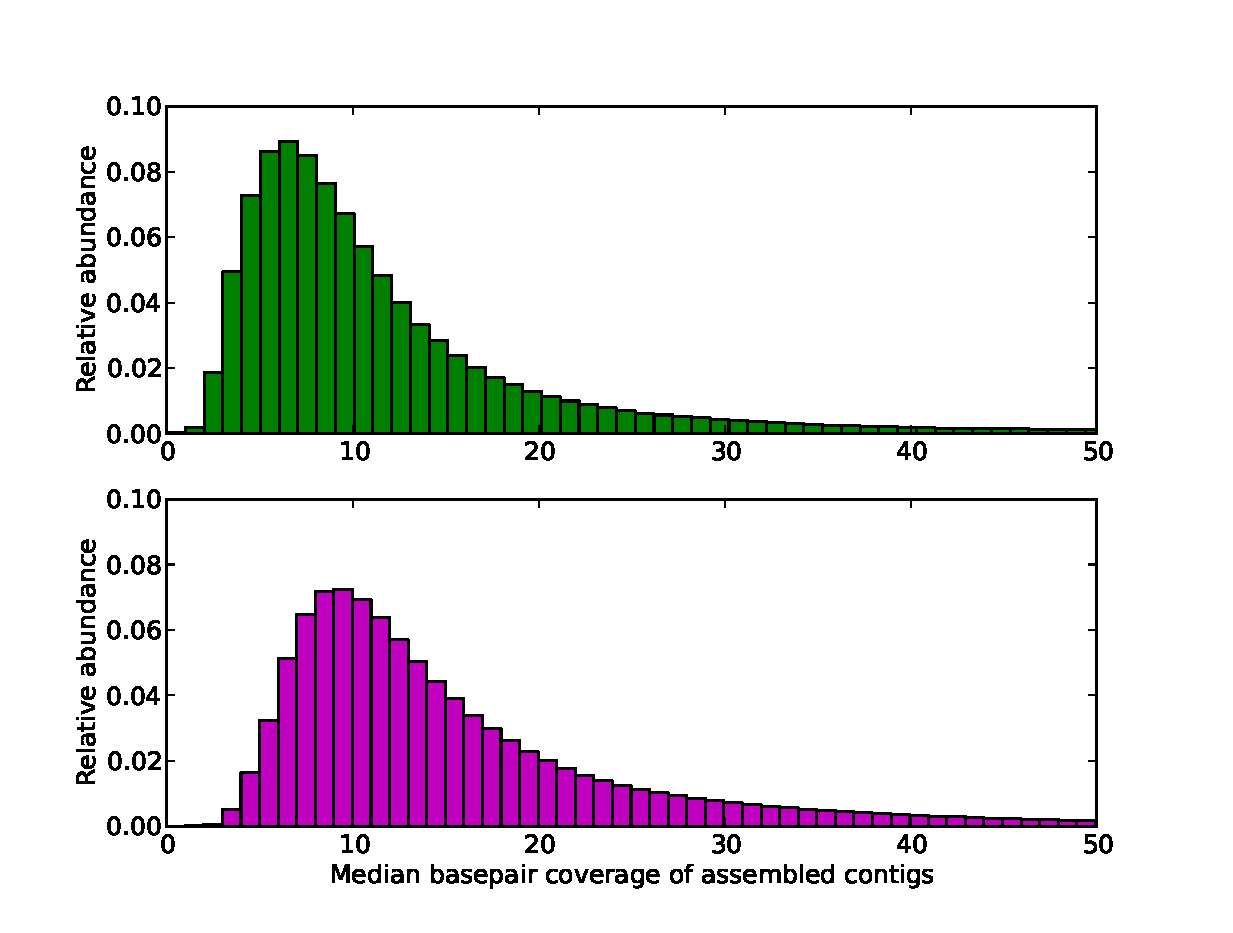
\includegraphics[width=.7\textwidth]{./figures/fig3-coverage.eps}}
\caption{Coverage (median basepair recovered) distribution of assembled contigs
from Iowa corn soil (top) and Iowa prairie soil (bottom) metagenomes.}
\label{soilassemblycoverage} \end{center} \end{figure}



\begin{figure}[ht] \begin{center}
\centerline{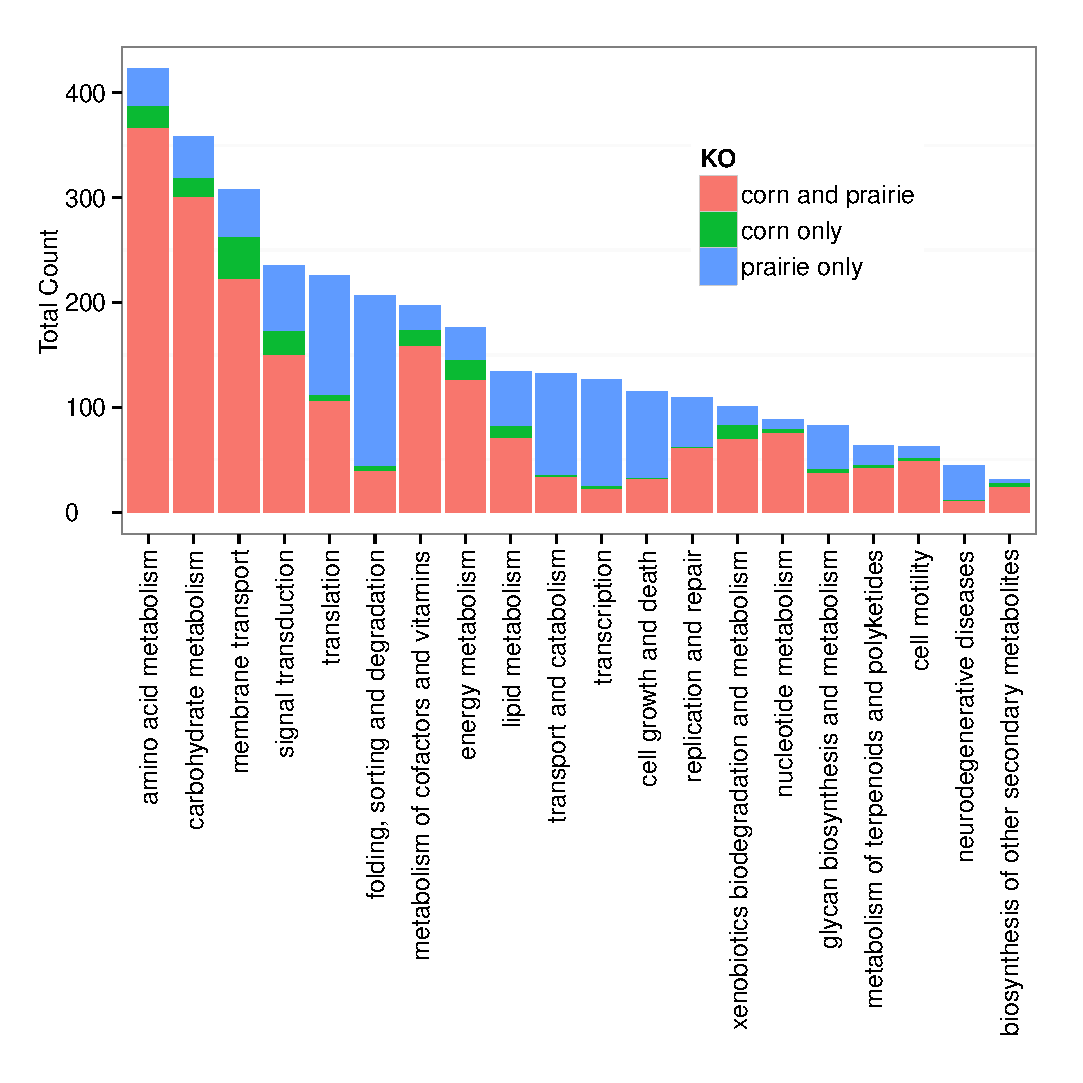
\includegraphics[width=.7\textwidth]{./figures/ko-distributions.eps}}
\caption{Distribution of most abundant KEGG Orthology groups identified in corn
and prairie soil metagenomes.} \label{kegg-dist} \end{center} \end{figure}



\begin{table} \caption{The total number of reads in unfiltered, normalized, and partitioned datasets and
the computational resources required (memory and time).}
\begin{tabular}{@{\extracolsep{\fill}}lccccc} 
\hline
& Unfiltered & Normalized & 
Partitioned \cr & Reads (Mbp) & Reads (Mbp) & Reads (Mbp) \cr \hline HMP Mock &
14,494,884 (1,136) & 8,656,520 (636) & 8,560,124 (631) \cr HMP Mock Spike &
14,992,845 (1,137) & 8,189,928 (612) & 8,094,475 (607) \cr HMP Mock Multispike &
17,010,607 (1,339) & 9,037,142 (702) & 8,930,840 (697) \cr Iowa Corn &
1,810,630,781 (140,750) & 1,406,361,241 (91,043) & 1,040,396,940 (77,603) \cr
Iowa Prairie & 3,303,375,485 (256,610) & 2,241,951,533 (144,962) & 1,696,187,797
(125,105) \cr \cr & Filter I: Normalization  & Filter II:  Partitioning & \cr &  (GB / h) &  (GB / h) \cr
HMP Mock & 4 / $<$2 & 4 / $<$2 \cr HMP Mock Spike & 4 / $<$2 & 4 / $<$2 \cr HMP
Mock Multispike & 4 / $<$2 & 4 / $<$2 \cr Iowa Corn & 188 / 83 & 234 / 120 \cr
Iowa Prairie & 258 / 178 & 287 / 310 \cr \hline \end{tabular}
\label{data-summary} \end{table}


\begin{table} \caption{Assembly summary statistics (total contigs, total million
bp assembly length, maximum contig size bp) of unfiltered, normalized filtered, 
or partitioned datasets with Velvet (V) assembler. Assembly for UF
and P datasets also shown for MetaIDBA (M) and SOAPdenovo(S) assemblers. Assemblies of Iowa
corn and prairie metagenomes could not be completed on unfiltered or normalized-only datasets.}
\begin{tabular} {@{\extracolsep{\fill}}lccccccccccc}
\hline
 & & Unfiltered & & & Normalized filtered & & & Partitioned & & Assembler \cr 
& \# Contigs & Length & Max. Contig & \# Contigs & Length & Max. Contig& \# Contigs & Length & Max. Contig \cr
\hline
HMP Mock & 29,063 & 38 & 146,795 & 30,082 & 35 & 90,497 & 30,115 & 35 & 90,497 & V \cr 
HMP Mock & 24,300 & 36 & 86,445 & - &-&-& 27,475 & 36 & 96,041 & M\cr 
HMP Mock & 36,689 & 37 & 32,736 & -&-&- & 29,295 & 37 & 58,598 & S \cr 
Iowa corn& - &-&-& -&-&- & 1,862,962 & 912& 20,234 & V \cr 
Iowa corn &- &- &- & -&-&- & 1,334,841 & 623 & 15,013 & M \cr 
Iowa corn & - &-&-& -&-&-& 1,542,436 & 675 & 15,075 & S \cr
Iowa prairie & - &-&-& -&-&- & 3,120,263 & 1,510 & 9,397 & V \cr 
Iowa prairie & - &-&-& -&-&- & 2,102,163 & 998 & 7,206 & M \cr 
Iowa prairie & -&-&- & -&-&- & 2,599,767 &1,145 & 5,423 & S \cr 
\hline 
\end{tabular} 
\label{assembly-summary} 
\end{table}


\begin{table} \caption{Unassembled reads (single-end (SE) and paired-end (PE)) mapped to Iowa corn and prairie Velvet assemblies.}
\begin{tabular}{@{\extracolsep{\fill}}lcc} 
\hline
& Iowa Corn Assembly & Iowa Prairie Assemby \cr \hline Total Unfiltered Reads & 1,810,630,781 & 3,303,375,485\cr
Total Unfiltered SE Reads & 141,517,075 & 358,817,057\cr SE aligned 1 time &
11,368,837 & 32,539,726\cr SE aligned $>$ 1 time & 562,637 & 1,437,284\cr \% SE
Aligned & 8.43\% & 9.47\% \cr Total Unfiltered PE Reads & 834,556,853 &
1,472,279,214\cr PE aligned 1 time & 54,731,320 & 110,353,902\cr PE aligned $>$
1 time &1,993,902 & 3,133,710\cr \% PE Aligned Disconcordantly & 0.47\% &
0.63\%\cr \% PE Aligned & 9.68\% & 11.20\%\cr \hline \end{tabular}
\label{read-map} \end{table}

\setcounter{figure}{0}
\setcounter{table}{0}
\renewcommand{\thepage}{S\arabic{page}}  
\renewcommand{\thesection}{S\arabic{section}}   
\renewcommand{\thetable}{S\arabic{table}}   
\renewcommand{\thefigure}{S\arabic{figure}}

\begin{figure}
\begin{center}
\centerline{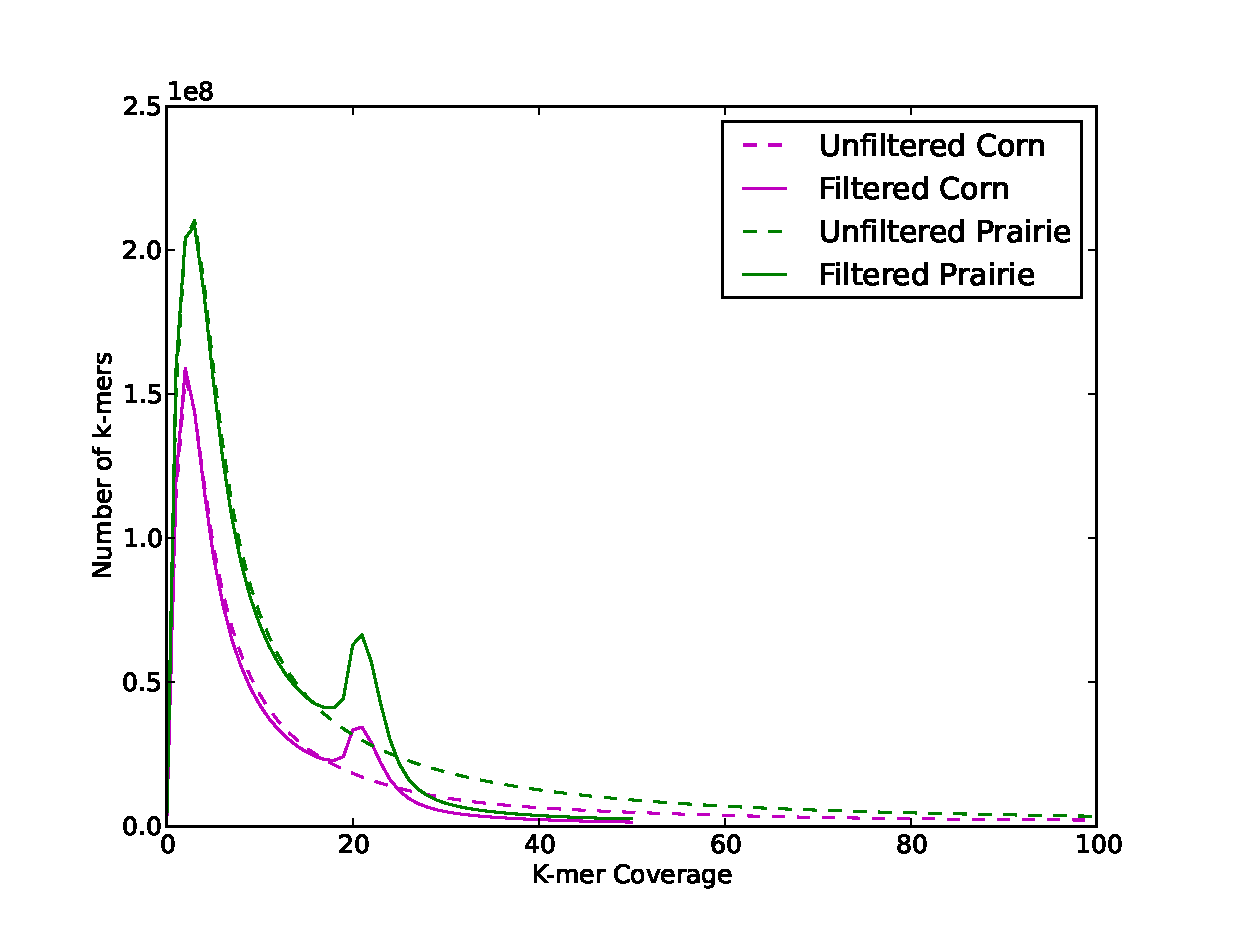
\includegraphics[width=.7\textwidth]{./figures/fig2-diginormhist.eps}}
\caption{K-mer coverage of Iowa corn and prairie metagenomes before
  and after normalization and partitioning filtering approaches.}
\label{diginormcoverage}
\end{center}
\end{figure}


\begin{figure}
\centerline{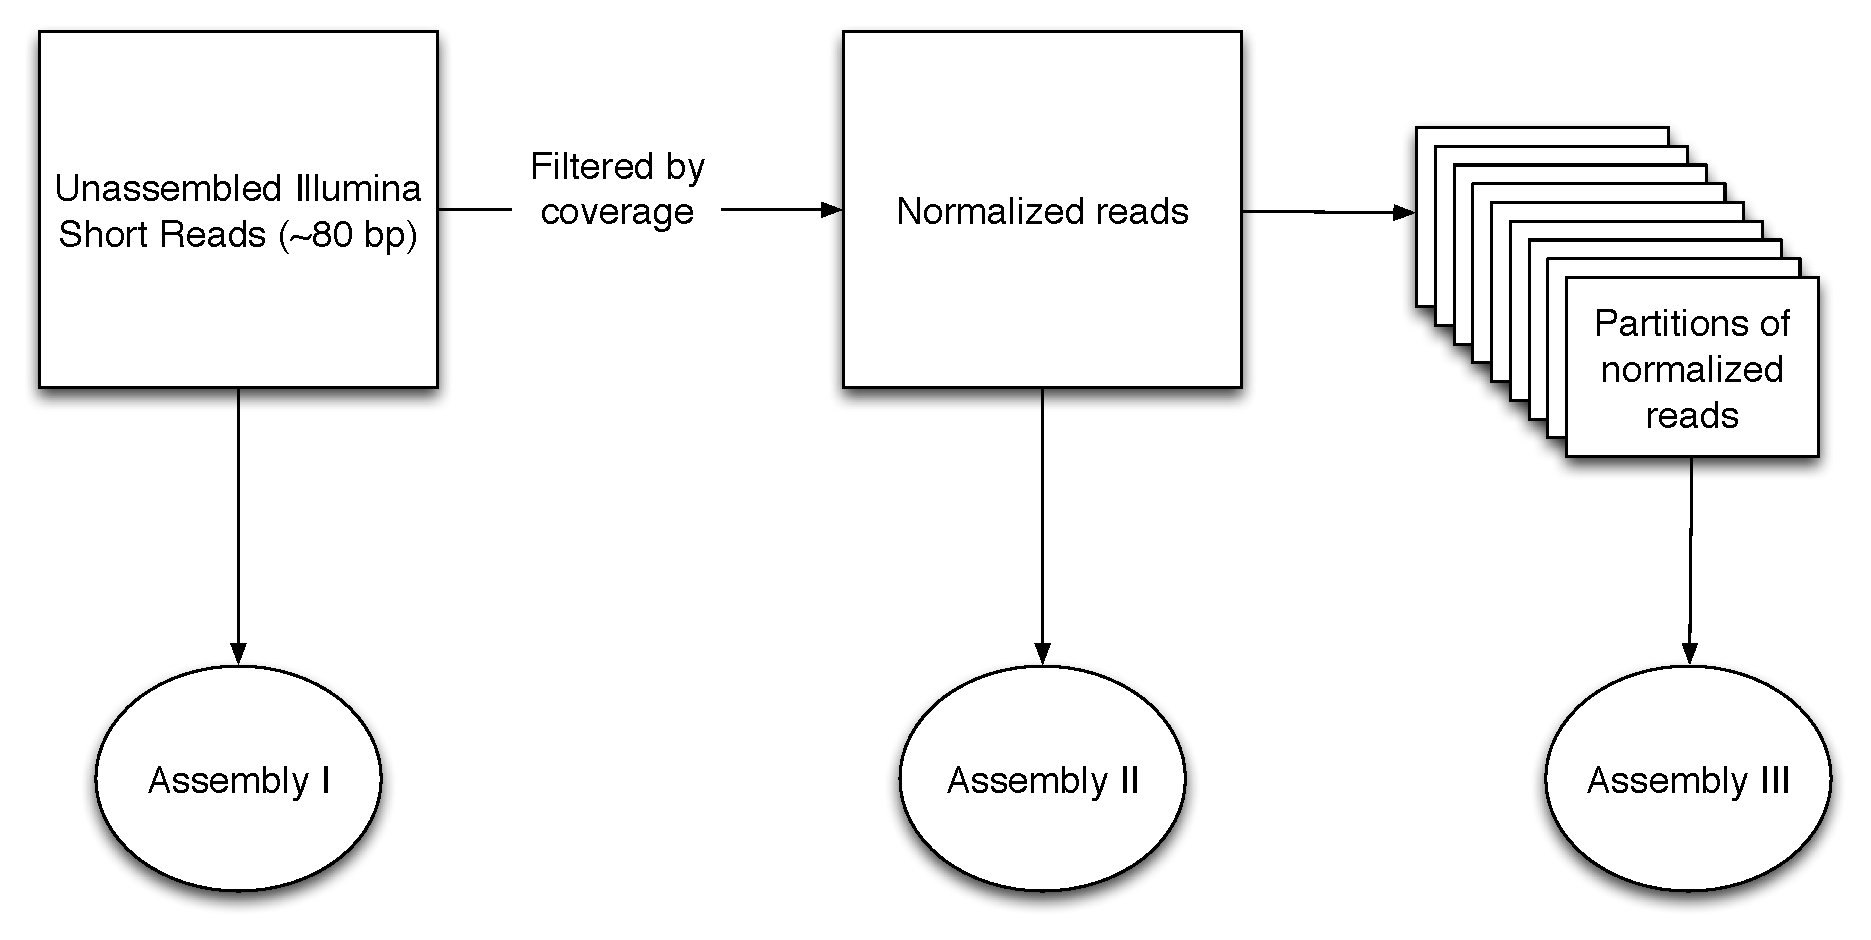
\includegraphics[width=.7\textwidth]{./figures/new_flowchart.eps}}
\caption{Unfiltered and filtered (by coverage) datasets and assemblies compared in this study.}
\label{flowchart}
\end{figure}

\begin{figure}
\centerline{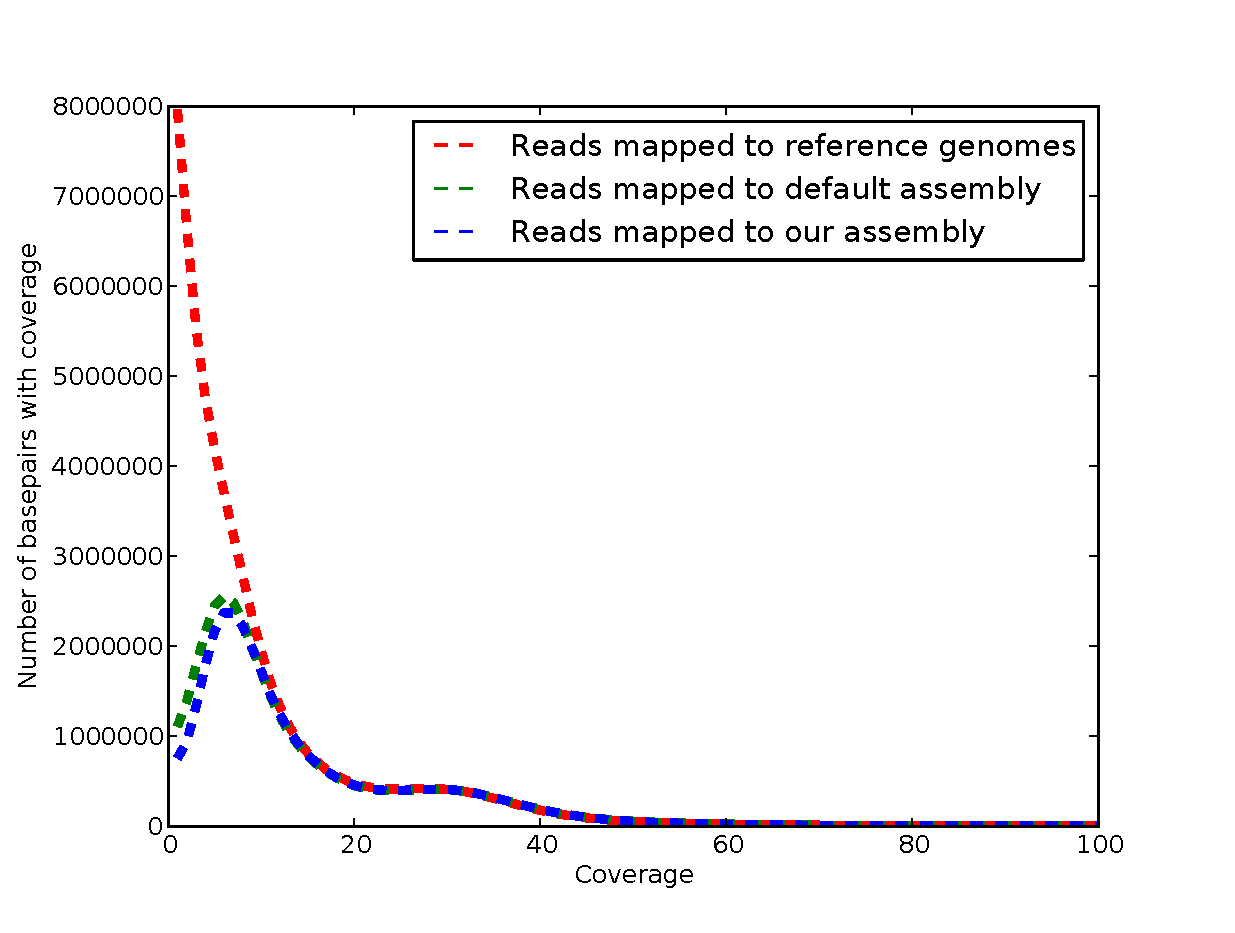
\includegraphics[width=.7\textwidth]{./figures/coverage.eps}}
\caption{For the HGMC datatset, the number of basepairs with specified coverage for reads which
  map to reference genomes and unfiltered and filtered assembled
  contigs greater than 300 bp.}
\label{coveragehmp}
\end{figure}

\begin{figure}
\center{\includegraphics[width=.7\textwidth]{./figures/reference_coverage.eps}}
\caption{Coverage of reference genomes (estimated actual coverage shown in parentheses) by sequences in unfiltered and normalized filtered unassembled reads and assembled contigs.}
\label{coverage1}
\end{figure}




\begin{figure}
\begin{center}
\centerline{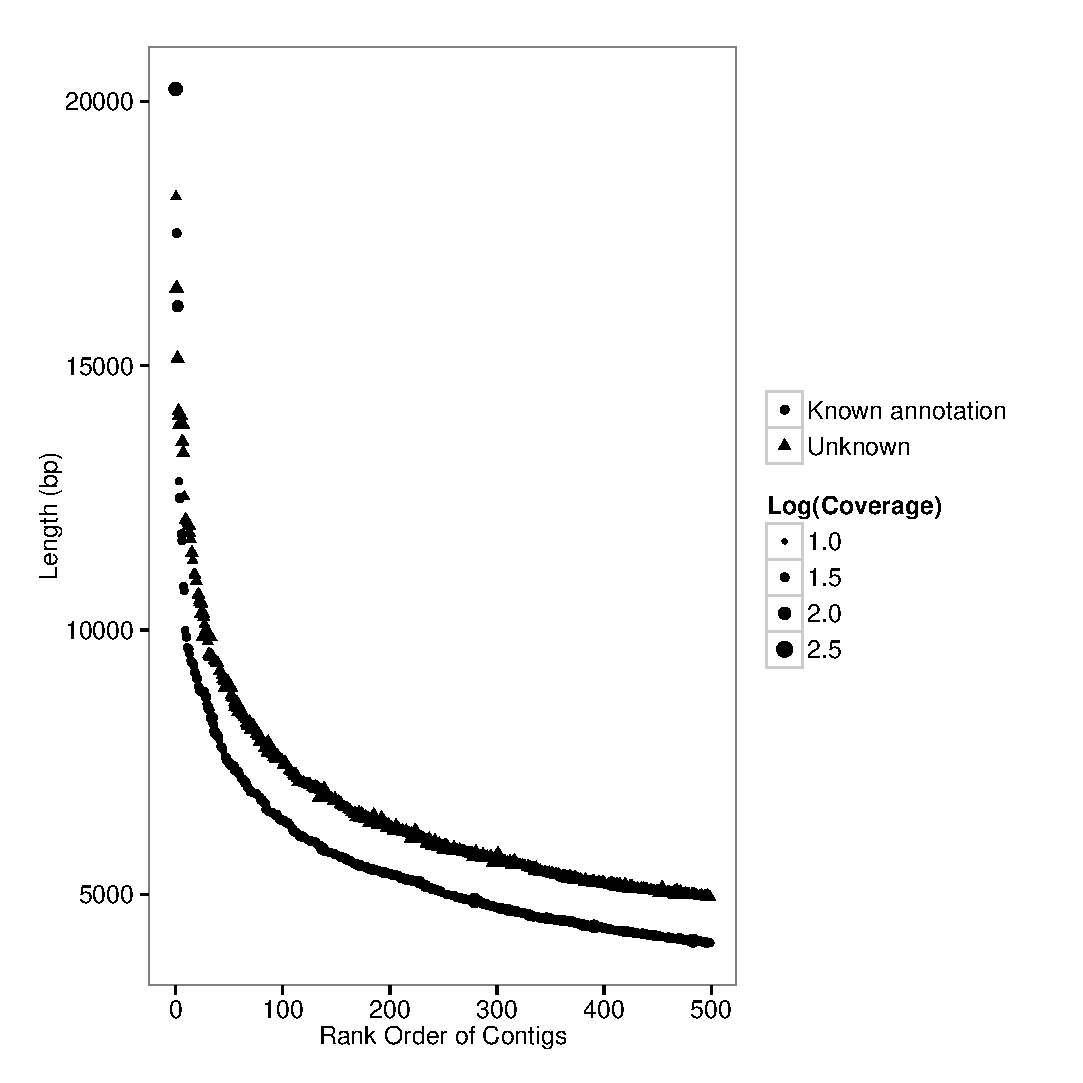
\includegraphics[width=.7\textwidth]{./figures/corn-cov-len-500.eps}}
\caption{Length distribution of longest assembled corn metagenome contigs with and without similarity to known sequences.  Unknown contigs were defined as sequences with no annotated gene regions.  Coverage (log-scale) of these sequences is also shown by the size of marker. }
\label{cornlength}
\end{center}
\end{figure}

\begin{figure}
\begin{center}
\centerline{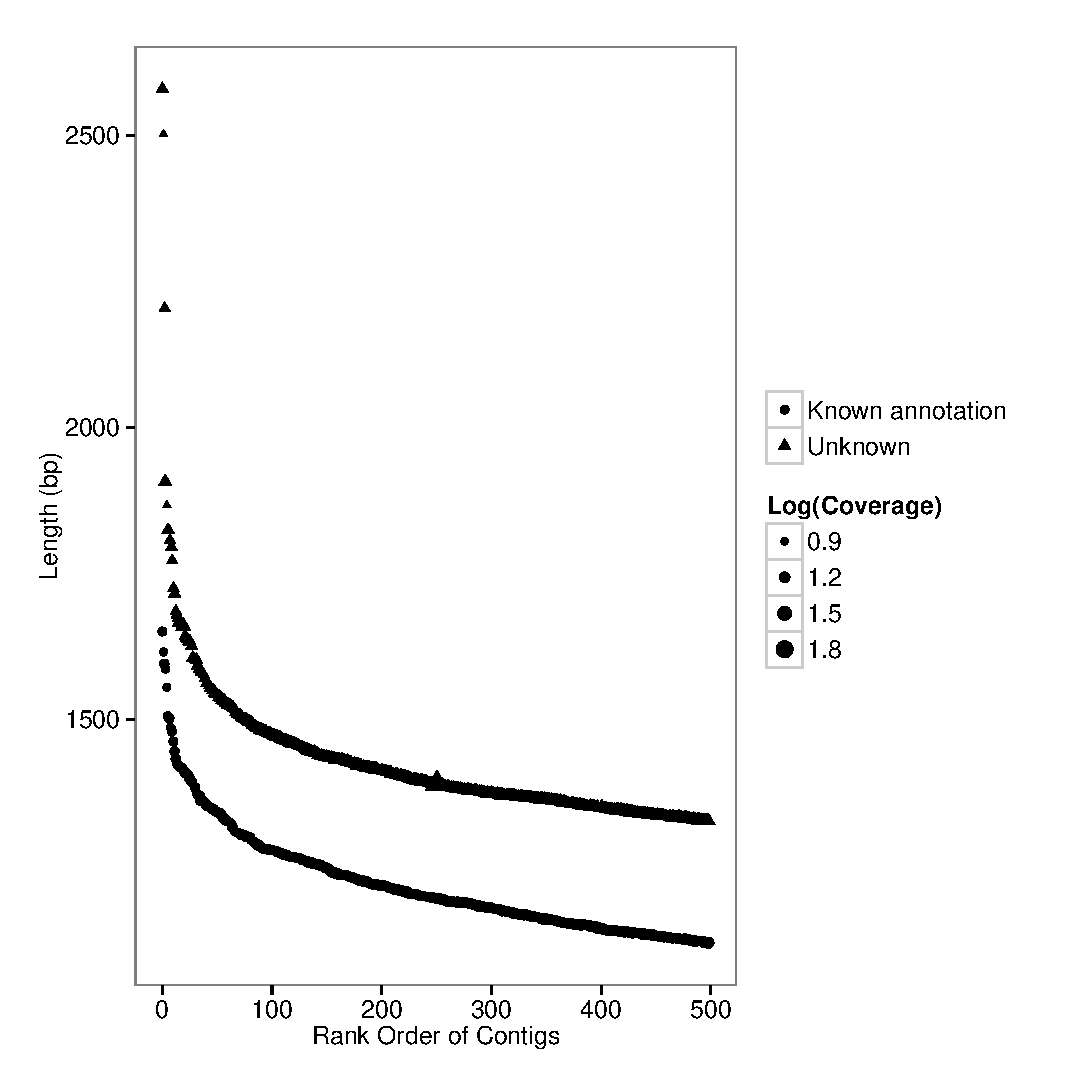
\includegraphics[width=.7\textwidth]{./figures/prairie-cov-len-500.eps}}
\caption{Length distribution of longest assembled prairie metagenome sequences with and without similarity to known sequences.  Coverage (log-scale) of these sequences is also shown by the size of marker. }
\label{prairielength}
\end{center}
\end{figure}


\begin{figure}
\begin{center}
\centerline{\includegraphics[width=.7\textwidth]{./figures/metabolism_kegg_pathway_all.eps}}
\caption{KEGG pathways sharing similarity with assembled soil metagenome sequences (black=combined corn and prairie, yellow = prairie only, orange = corn only.}
\label{kegg}
\end{center}
\end{figure}


\begin{table}
\caption{Assembly comparisons of unfiltered (UF) and normalized filtered (NF) or
  filtered/partitioned (FP) HMP mock datasets using different
  assemblers (Velvet (V), MetaIDBA (M) and SOAPdenovo (S)).  Assembly
  content similarity is based on the fraction of alignment of
  assemblies and similarly, the coverage of reference genomes is based
  on the alignment of assembled contigs to reference genomes (RG).}
\begin{tabular}{@{\extracolsep{\fill}}lcccc}
Assembly Comparison & Percent Similarity & RG Coverage & Assembler \\
\hline
UF vs. NF & 95\% & 43.3\% / 44.5\% & V \\
UF vs. FP & 95\% & 43.3\% / 44.4\% & V\\
UF vs. FP & 93\% & 46.5\% / 45.4\% & M\\ 
UF vs. FP & 98\% &  46.2\% / 46.4\% & S\\
\hline
\end{tabular}
\label{assembly-compare}
\end{table}


\begin{table}
\caption{HMP mock dataset reference genomes estimated sequencing depth
  (median bp coverage of reads), number of partitions, total length
  (bp), coverage of reference genomes by unfiltered reads (UF Cov),
  coverage of reference genomes by normalized filtered reads (F Cov), coverage of
  reference genomes by unfiltered assembled contigs (UFA Cov), and
  coverage of reference genomes by normalized filtered assembled contigs (FA
  Cov).}
\begin{tabular}{@{\extracolsep{\fill}}l c c c c c c c}
\hline Reference Genome & Coverage & No. Partitions & Length (bp) & UF
Cov (bp) & F Cov (bp) & UFA Cov & FA Cov \\ \hline
gi\textbar{}32470588\textbar{}ref\textbar{}NC\_005008.1\textbar{} &
2,412 & 9 & 4,439 & 4,439 & 1,058 & 100 \% & 28 \% \\
gi\textbar{}32470581\textbar{}ref\textbar{}NC\_005007.1\textbar{} &
549 & 16 & 4,679 & 4,679 & 4,585 & 100 \% & 77 \% \\
gi\textbar{}32470520\textbar{}ref\textbar{}NC\_005003.1\textbar{} &
533 & 21 & 6,585 & 6,585 & 6,441 & 100 \% & 64 \% \\
gi\textbar{}32470572\textbar{}ref\textbar{}NC\_005006.1\textbar{} &
253 & 2 & 8,007 & 8,004 & 7,953 & 100 \% & 100 \% \\
gi\textbar{}32470532\textbar{}ref\textbar{}NC\_005004.1\textbar{} &
112 & 52 & 24,365 & 24,358 & 24,291 & 100 \% & 83 \% \\
gi\textbar{}126640109\textbar{}ref\textbar{}NC\_009084.1\textbar{} &
85 & 3 & 11,302 & 11,295 & 11,270 & 100 \% & 100 \% \\
gi\textbar{}32470555\textbar{}ref\textbar{}NC\_005005.1\textbar{} & 74
& 12 & 17,261 & 17,202 & 17,180 & 100 \% & 100 \% \\
gi\textbar{}10957398\textbar{}ref\textbar{}NC\_000958.1\textbar{} & 71
& 73 & 177,466 & 177,261 & 174,614 & 100 \% & 95 \% \\
gi\textbar{}10957530\textbar{}ref\textbar{}NC\_000959.1\textbar{} & 52
& 37 & 45,704 & 44,974 & 43,557 & 100 \% & 92 \% \\
gi\textbar{}126640097\textbar{}ref\textbar{}NC\_009083.1\textbar{} &
48 & 2 & 13,408 & 13,405 & 13,383 & 100 \% & 100 \% \\
gi\textbar{}15807672\textbar{}ref\textbar{}NC\_001264.1\textbar{} & 40
& 63 & 412,348 & 410,970 & 403,553 & 100 \% & 99 \% \\
gi\textbar{}15805042\textbar{}ref\textbar{}NC\_001263.1\textbar{} & 32
& 546 & 2,648,638 & 2,634,512 & 2,589,566 & 100 \% & 99 \% \\
gi\textbar{}27466918\textbar{}ref\textbar{}NC\_004461.1\textbar{} & 30
& 476 & 2,499,279 & 2,498,081 & 2,492,248 & 100 \% & 98 \% \\
gi\textbar{}125654693\textbar{}ref\textbar{}NC\_009008.1\textbar{} &
29 & 14 & 37,100 & 36,585 & 33,250 & 94 \% & 96 \% \\
gi\textbar{}161508266\textbar{}ref\textbar{}NC\_010079.1\textbar{} &
29 & 442 & 2,872,915 & 2,298,758 & 2,157,196 & 100 \% & 92 \% \\
gi\textbar{}77404776\textbar{}ref\textbar{}NC\_007490.1\textbar{} & 27
& 27 & 100,828 & 99,385 & 93,550 & 100 \% & 96 \% \\
gi\textbar{}125654605\textbar{}ref\textbar{}NC\_009007.1\textbar{} &
24 & 92 & 114,045 & 108,526 & 97,860 & 100 \% & 96 \% \\
gi\textbar{}77404693\textbar{}ref\textbar{}NC\_007489.1\textbar{} & 18
& 12 & 105,284 & 102,212 & 96,169 & 100 \% & 99 \% \\
gi\textbar{}24378532\textbar{}ref\textbar{}NC\_004350.1\textbar{} & 16
& 131 & 2,030,921 & 2,029,376 & 2,025,544 & 100 \% & 99 \% \\
gi\textbar{}77404592\textbar{}ref\textbar{}NC\_007488.1\textbar{} & 13
& 30 & 114,178 & 103,351 & 93,637 & 100 \% & 99 \% \\
gi\textbar{}77461965\textbar{}ref\textbar{}NC\_007493.1\textbar{} & 13
& 628 & 3,188,609 & 2,919,441 & 2,681,855 & 100 \% & 99 \% \\
gi\textbar{}77464988\textbar{}ref\textbar{}NC\_007494.1\textbar{} & 13
& 262 & 943,016 & 862,781 & 788,626 & 100 \% & 98 \% \\
gi\textbar{}126640115\textbar{}ref\textbar{}NC\_009085.1\textbar{} &
11 & 683 & 3,976,747 & 3,939,190 & 3,936,208 & 99 \% & 99 \% \\
gi\textbar{}148642060\textbar{}ref\textbar{}NC\_009515.1\textbar{} & 9
& 552 & 1,853,160 & 1,828,231 & 1,826,639 & 99 \% & 98 \% \\
gi\textbar{}150002608\textbar{}ref\textbar{}NC\_009614.1\textbar{} & 7
& 7,751 & 5,163,189 & 4,899,622 & 4,896,808 & 81 \% & 82 \% \\
gi\textbar{}15644634\textbar{}ref\textbar{}NC\_000915.1\textbar{} & 6
& 2,888 & 1,667,867 & 1,581,502 & 1,581,024 & 78 \% & 79 \% \\
gi\textbar{}194172857\textbar{}ref\textbar{}NC\_003028.3\textbar{} & 6
& 4,123 & 2,160,842 & 2,047,832 & 2,037,347 & 78 \% & 78 \% \\
gi\textbar{}49175990\textbar{}ref\textbar{}NC\_000913.2\textbar{} & 6
& 5,913 & 4,639,675 & 4,080,605 & 4,074,119 & 84 \% & 85 \% \\
gi\textbar{}50841496\textbar{}ref\textbar{}NC\_006085.1\textbar{} & 6
& 6,459 & 2,560,265 & 2,169,547 & 2,169,056 & 59 \% & 64 \% \\
gi\textbar{}77358697\textbar{}ref\textbar{}NC\_003112.2\textbar{} & 4
& 9,269 & 2,272,360 & 1,655,023 & 1,626,301 & 28 \% & 33 \% \\
\hline
\end{tabular}
\label{ref-summary}
\end{table}


\begin{table}
\caption{Longest contigs in the corn and prairie soil metagenome with similarity to the RefSeq database. (*Indicates SEED database origin if no RefSeq organismal annotaiton available.)}
\begin{tabular}{@{\extracolsep{\fill}}lccl}
Contig ID & Length (bp) & Coverage &  Function \& Organsim \\
 \hline
iowa-corn-3-pass.4582796.20234*	&	20234	&	138	&	Probable poly(beta-D-mannuronate) O-acetylase (EC 2.3.1.-)	\\
	&		&		&	Cyanothece sp PCC 7425	\\
iowa-corn-3-pass.4606542.17507	&	17507	&	30	&	hypothetical protein	\\
	&		&		&	Pseudomonas phage PaP2	\\
iowa-corn-3-pass.4578484.16126	&	16126	&	62	&	hypothetical protein	\\
	&		&		&	Pseudomonas phage PaP2	\\
iowa-corn-3-pass.4583611.12814	&	12814	&	18	&	replication factor C large subunit	\\
	&		&		&	Candidatus Methanoregula boonei 6A8	\\
iowa-corn-3-pass.4594771.12496	&	12496	&	35	&	carbonic anhydrase	\\
	&		&		&	Psychromonas ingrahamii 37	\\
iowa-corn-3-pass.4596152.11816	&	11816	&	25	&	ribonuclease Z	\\
	&		&		&	Thermococcus kodakarensis KOD1	\\
iowa-corn-3-pass.4616349.11691	&	11691	&	25	&	precorrin-3B C17-methyltransferase	\\
	&		&		&	Nitrosopumilus maritimus SCM1	\\
iowa-corn-3-pass.4592007.10823	&	10823	&	22	&	hydroxymethylglutaryl-CoA reductase, degradative	\\
	&		&		&	Staphylothermus marinus F1	\\
iowa-corn-3-pass.4589906.10747	&	10747	&	23	&	RdgB/HAM1 family non-canonical purine NTP pyrophosphatase	\\
	&		&		&	Roseiflexus castenholzii DSM 13941	\\
iowa-corn-3-pass.4559414.9998&	9998	&	19	&	heparan N-sulfatase	\\
	&		&		&	Blastopirellula marina DSM 3645	\\
iowa-prairie-3-pass.6326293.1650	&	1650	&	11	&	PAS/PAC sensor signal transduction histidine kinase	\\
	&		&		&	Marinobacter aquaeolei VT8	\\
iowa-prairie-3-pass.6215171.1615*	&	1615	&	9	&	Beta-mannosidase (EC 3.2.1.25)	\\
	&		&		&	Acidobacteria bacterium Ellin345	\\
iowa-prairie-3-pass.6327344.1595	&	1595	&	12	&	glycosyl transferase, group 2 family protein	\\
	&		&		&	Bacillus cereus ATCC 10987	\\
iowa-prairie-3-pass.6326016.1586	&	1586	&	10	&	hypothetical protein	\\
	&		&		&	Dechloromonas aromatica RCB	\\
iowa-prairie-3-pass.6155396.1555	&	1555	&	9	&	peptidase S33, proline iminopeptidase 1	\\
	&		&		&	Pseudomonas syringae pv. syringae B728a	\\
iowa-prairie-3-pass.6285889.1505	&	1505	&	11	&	AMP-dependent synthetase and ligase	\\
	&		&		&	Chloroflexus sp. Y-400-fl	\\
iowa-prairie-3-pass.6293899.1502	&	1502	&	13	&	beta-lactamase	\\
	&		&		&	Flavobacterium johnsoniae UW101	\\
iowa-prairie-3-pass.5906709.1488	&	1488	&	7	&	peptidase M24	\\
	&		&		&	Chitinophaga pinensis DSM 2588	\\
iowa-prairie-3-pass.6216765.1484	&	1484	&	10	&	amine oxidase	\\
	&		&		&	Candidatus Solibacter usitatus Ellin6076	\\
iowa-prairie-3-pass.6224149.1479	&	1479	&	12	&	phosphoribosylglycinamide formyltransferase 	\\
& & & Bacteroides sp. 2\_1\_16\\
\hline
\end{tabular}
\label{mgrast}
\end{table}


\end{document}
% LocalWords: situ ultradeep Tbp dataset metagenomic metagenome
Gbp NCBI novo % LocalWords: RefSeq metagenomes contigs
